\subsection{Introduction}

CLIP (Radford et al., 2021) applies contrastive representation learning
across modalities: an image encoder and a text encoder are trained jointly
so that an image's embedding and its matching caption's embedding land close
together in a shared space, while embeddings of mismatched image/caption
pairs are pushed apart. This section investigates three consequences of that
design, all now measured empirically on \texttt{ViT-B/32} CLIP and STL-10:
whether the resulting shared space supports zero-shot classification under
three prompting strategies of increasing linguistic richness; whether the
two modalities' embeddings actually occupy the same region of that shared
space or a measurably separated one (the ``modality gap''); and whether a
simple rigid-rotation alignment can close that gap and improve zero-shot
accuracy.

\subsection{Methodology}

\subsubsection{Contrastive Pretraining and InfoNCE}

Directly maximizing the mutual information $I(X;Z)$ between an input $X$
and a representation $Z=f(X)$ is intractable for high-dimensional data, since
it requires density estimates that are unavailable. Contrastive learning
sidesteps this by turning representation learning into a classification
problem: given an anchor and a batch of candidates (one positive, many
negatives), train an encoder to identify the positive. The InfoNCE loss,
\[
  \mathcal{L}_{\text{InfoNCE}} = -\mathbb{E}\left[\log\frac{f(x_{\text{pos}},c)}{\sum_j f(x_j,c)}\right],
\]
satisfies $I(x;c)\geq\log N - \mathcal{L}_{\text{InfoNCE}}$: minimizing
InfoNCE maximizes a lower bound on mutual information, so ``can you pick the
correct pair out of a batch of distractors'' is a tractable proxy for ``does
this representation preserve the information that matters.''

\subsubsection{CLIP: Cross-Modal Contrastive Pretraining}
\label{sec:clip-methodology}

CLIP applies this InfoNCE-style objective \emph{across} modalities rather
than within one. For a batch of $B$ image/text pairs, with $\hat{x}_i,
\hat{y}_i\in\mathcal{S}^{d-1}$ the L2-normalized image and text embeddings
and temperature $\tau$, CLIP minimizes the symmetric average of the
image-to-text and text-to-image directions,
\[
  \mathcal{L}_{v\to t} = -\frac{1}{B}\sum_{i=1}^B\log\frac{\exp(\langle\hat{x}_i,\hat{y}_i\rangle/\tau)}{\sum_{j=1}^B\exp(\langle\hat{x}_i,\hat{y}_j\rangle/\tau)},
\]
\[
  \mathcal{L}_{t\to v} = -\frac{1}{B}\sum_{i=1}^B\log\frac{\exp(\langle\hat{x}_i,\hat{y}_i\rangle/\tau)}{\sum_{j=1}^B\exp(\langle\hat{x}_j,\hat{y}_i\rangle/\tau)},
\]
\[
  \mathcal{L}_{\text{CLIP}} = \tfrac{1}{2}(\mathcal{L}_{v\to t}+\mathcal{L}_{t\to v}).
\]
Zero-shot classification follows directly from this objective: given
candidate class descriptions $y_1,\dots,y_C$,
$\hat{c}=\arg\max_c\langle\hat{f}_v(x),\hat{f}_t(y_c)\rangle$ -- no
classification head, no fine-tuning.

\subsubsection{Zero-Shot Classification Protocol (Task 3.1)}

\texttt{ViT-B/32} CLIP is evaluated on the full STL-10 test set (8000
images, 10 classes) under three prompting strategies: plain labels (e.g.\
``airplane''), a fixed template (``a photo of an airplane.''), and a more
descriptive hand-written variant (``a high-quality, clear photo of an
airplane, prominently visible in the center of the frame.''). Since only
the text side changes across strategies, the 8000 test images are encoded
once and reused against each strategy's 10 text embeddings.

\subsubsection{Modality Gap Protocol (Task 3.2)}

Image and text embeddings for 100 paired STL-10 samples ($d=512$) are
jointly projected to 2D via UMAP, once on raw embeddings and once on
L2-normalized embeddings. A centroid-distance metric,
$\Delta_{\text{gap}}=\|\mu_v-\mu_t\|_2$ with
$\mu_v=\frac{1}{N}\sum_i\hat{x}_i$, $\mu_t=\frac{1}{N}\sum_i\hat{y}_i$,
quantifies the separation between the two modalities' embedding clouds.

\subsubsection{Procrustes Alignment Protocol (Task 3.3)}

An orthogonal matrix $R\in\mathcal{O}(d)$ (satisfying $R^\top R=I$) is fit
via SciPy's \texttt{orthogonal\_procrustes} function on the same 100 paired
embeddings to solve $\min_R\|XR-Y\|_F^2$, with closed-form solution
$R^*=UV^\top$ from the SVD $X^\top Y=U\Sigma V^\top$. Because $R$ is a
single global $512\times512$ rotation rather than a sample-specific
transform, it is fit on the 100-pair subset and applied to all 8000
test-image embeddings. Zero-shot accuracy is recomputed on the rotated
embeddings for all three prompting strategies and compared against the
Task 3.1 baseline.

\subsection{Results}

\subsubsection{Zero-Shot Classification}

\begin{table}[t]
\centering
\caption{Zero-shot accuracy on the full STL-10 test set (8000 images), by prompting strategy.}
\label{tab:clip-prompts}
\begin{tabular}{lc}
\hline
Strategy & Accuracy \\
\hline
Plain (``airplane'') & 96.25\% \\
Templated (``a photo of an airplane.'') & \textbf{97.29\%} \\
Descriptive & 96.29\% \\
\hline
\end{tabular}
\end{table}

Table~\ref{tab:clip-prompts} shows the templated prompt achieves the
highest accuracy, $1.04$ points above plain labels. The descriptive prompt
underperforms the template by $1.00$ point, landing almost exactly at the
plain-label accuracy despite containing more information about the target
class.

\subsubsection{Modality Gap}

\begin{figure}[t]
\centering
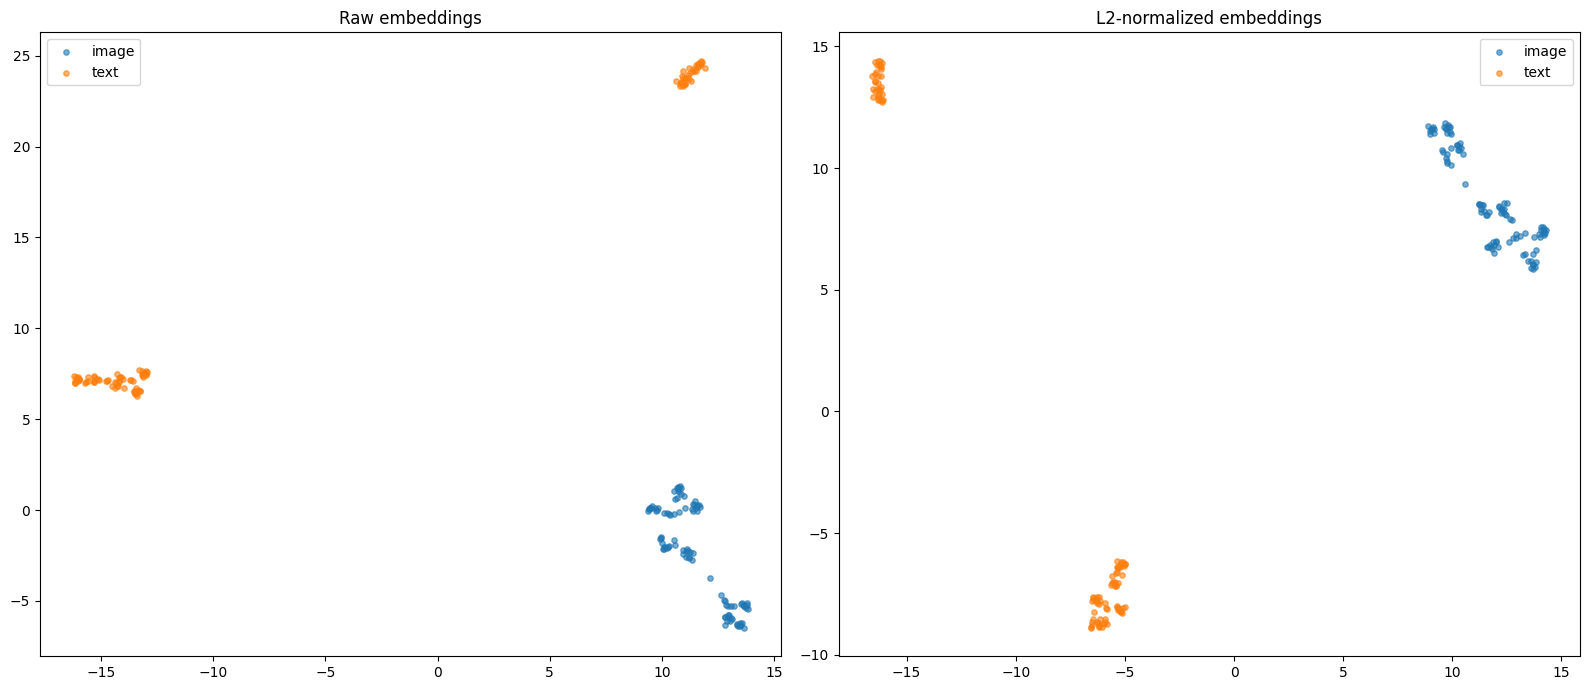
\includegraphics[width=\linewidth]{assets/clip_fig1.png}
\caption{UMAP projection of 100 paired image/text embeddings: raw (left) vs.\ L2-normalized (right).}
\label{fig:clip-gap}
\end{figure}

In both the raw and normalized projections (Figure~\ref{fig:clip-gap}),
image embeddings and text embeddings form visibly separate clusters with
no interleaving. The measured centroid distance in the normalized,
$512$-dimensional space is $\Delta_{\text{gap}}=1.0495$.

\subsubsection{Procrustes Alignment}

\begin{figure}[t]
\centering
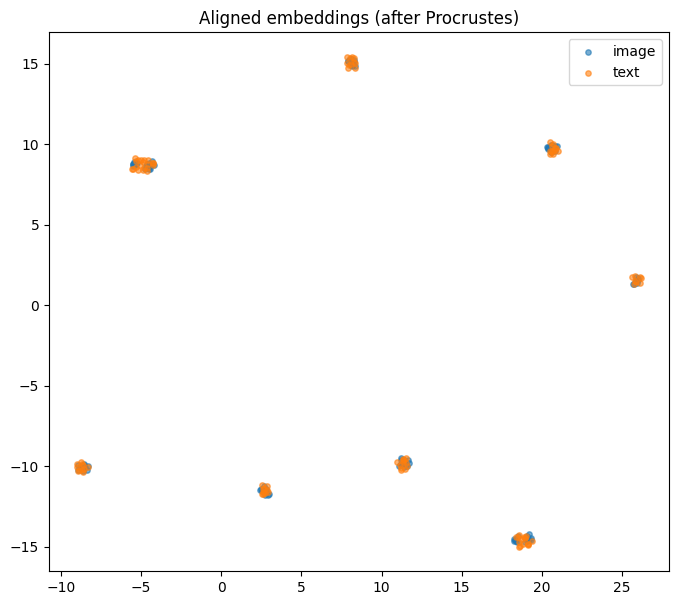
\includegraphics[width=0.85\linewidth]{assets/clip_fig2.png}
\caption{UMAP projection of the 100 paired embeddings after orthogonal Procrustes alignment.}
\label{fig:clip-aligned}
\end{figure}

\begin{table}[t]
\centering
\caption{Zero-shot accuracy before vs.\ after Procrustes alignment.}
\label{tab:clip-aligned}
\begin{tabular}{lccc}
\hline
Strategy & Baseline & Aligned & $\Delta$ \\
\hline
Plain & 96.25\% & 96.00\% & $-0.25$ \\
Templated & 97.29\% & 97.16\% & $-0.13$ \\
Descriptive & 96.29\% & 96.38\% & $+0.09$ \\
\hline
\end{tabular}
\end{table}

The fitted rotation $R$ is confirmed orthogonal ($R^\top R\approx I$) and
norm-preserving (embedding norms $1.0000$ before and after). Alignment
reduces the centroid distance by $87.3\%$, from $\Delta_{\text{gap}}=1.0495$
to $\Delta_{\text{aligned}}=0.1326$ -- visually confirmed in
Figure~\ref{fig:clip-aligned}, where image and text points now sit
essentially on top of each other within each cluster, in sharp contrast to
Figure~\ref{fig:clip-gap}'s two separated clouds. Despite this large
geometric change, zero-shot accuracy is essentially unchanged: all three
strategies shift by at most a quarter of a percentage point
(Table~\ref{tab:clip-aligned}), with no consistent direction (plain and
templated go slightly down, descriptive slightly up).

\subsection{Discussion}

\subsubsection{Why Templated Prompts Win, and Why More Description Does Not Help Further}

CLIP's text encoder was trained on naturally-occurring web captions --
full sentences, not bare category words -- via the InfoNCE objective in
Section~\ref{sec:clip-methodology}. A bare label like ``airplane'' provides no sentence context,
placing it out-of-distribution relative to what the text encoder saw
during training; embedding it into a standard template
(``a photo of an airplane.'') moves it back into the natural distribution
of CLIP's shared space, which is the direct explanation for the $+1.04$
point gain over plain labels observed in Table~\ref{tab:clip-prompts}. The
descriptive prompt's underperformance \emph{relative to the template} is
the more interesting result: with a long, generic prefix (``a
high-quality, clear photo of...''), the transformer's self-attention has
more filler tokens to distribute weight across, diluting the effective
attention mass on the class-identifying token itself. The net effect very
nearly cancels the distributional benefit of using a full sentence at all,
landing the descriptive prompt within $0.04$ points of the plain-label
baseline -- consistent with two competing effects (in-distribution
phrasing helps; attention dilution from excess wording hurts) that happen
to roughly offset for this particular prompt.

\subsubsection{Why the Modality Gap Persists Under L2-Normalization}

L2-normalization constrains both modalities to the surface of the unit
hypersphere $\mathcal{S}^{d-1}$, which makes squared Euclidean distance a
monotonic function of cosine similarity,
$\|\hat{x}-\hat{y}\|_2^2=2-2\langle\hat{x},\hat{y}\rangle$ -- but nothing
about this constraint forces the two modalities' \emph{directions} on that
sphere to coincide. That the measured gap survives normalization almost
unchanged confirms this is a genuine angular separation (an image-cone and
a text-cone occupying disjoint sectors of the sphere), not merely a
radial/scale artifact that normalization would have removed. The root
cause is what InfoNCE actually optimizes: it enforces only that
$\langle\hat{x}_i,\hat{y}_i\rangle>\langle\hat{x}_i,\hat{y}_j\rangle$ for
$j\neq i$ within a batch -- a relative-ranking constraint -- with no term
rewarding $\|\hat{x}-\hat{y}\|\to0$ for matched pairs or penalizing
separation between the two modalities' overall clouds. The measured
$\Delta_{\text{gap}}=1.0495$ (out of a maximum possible distance of $2$ on
the unit sphere) is the empirical signature of that missing constraint.

\subsubsection{Why Zero-Shot Classification Survives a Large Modality Gap}

Modeling the gap as a shared, roughly class-invariant offset per modality,
$\hat{x}\approx z_i+\delta_v$ and $\hat{y}_c\approx z_c+\delta_t$, the
classification rule expands to
\[
  \begin{aligned}
  \arg\max_c\langle\hat{x},\hat{y}_c\rangle
  = \arg\max_c\big[&\langle z_i,z_c\rangle+\langle z_i,\delta_t\rangle \\
  &+\langle\delta_v,z_c\rangle+\langle\delta_v,\delta_t\rangle\big].
  \end{aligned}
\]
Since $\delta_t$ is approximately the same across all candidate text
prompts for a fixed image, the $\langle z_i,\delta_t\rangle$ and
$\langle\delta_v,\delta_t\rangle$ terms are (to first order) constant
across the $\arg\max$ over $c$, and $\langle\delta_v,z_c\rangle$ shifts all
classes similarly rather than reordering them. Table~\ref{tab:clip-aligned}
is the direct empirical test of this argument: even though alignment
removes $87.3\%$ of $\Delta_{\text{gap}}$ (i.e.\ removes most of exactly
the $\delta_v,\delta_t$ structure this argument treats as
classification-irrelevant), accuracy barely moves. This is strong evidence
that the offset-invariance model is essentially correct for this data, not
just a plausible-sounding approximation.

\subsubsection{Procrustes Alignment: Large Geometric Effect, Negligible Accuracy Effect}

Because $R$ is constrained to be orthogonal, it is an isometry
($\|xR\|_2=\|x\|_2$ and $\langle x_iR,x_jR\rangle=\langle x_i,x_j\rangle$
for any $x_i,x_j$) -- confirmed directly in the implementation
($R^\top R\approx I$, embedding norms unchanged at $1.0000$). It can only
rotate the image-embedding cloud rigidly toward the text cloud; it cannot
distort either modality's internal geometry to artificially minimize the
alignment objective. This isometry property is exactly why the two results
in this section are simultaneously true and mutually consistent rather
than contradictory: the rotation dramatically shrinks the \emph{absolute}
separation between the two clouds ($87.3\%$ reduction in centroid
distance, visually obvious in Figure~\ref{fig:clip-aligned}), while
leaving all pairwise angles -- and therefore the $\arg\max_c$ ranking that
zero-shot classification actually depends on -- essentially untouched.
Absolute spatial proximity between modalities and downstream zero-shot
discriminability are, empirically, decoupled quantities: closing the
modality gap is not, in itself, what makes CLIP's zero-shot classification
work.
